% Options for packages loaded elsewhere
\PassOptionsToPackage{unicode}{hyperref}
\PassOptionsToPackage{hyphens}{url}
\PassOptionsToPackage{dvipsnames,svgnames,x11names}{xcolor}
%
\documentclass[
  sigconf]{acmart}
\usepackage{amsmath}
\usepackage{lmodern}
\usepackage{iftex}
\ifPDFTeX
  \usepackage[T1]{fontenc}
  \usepackage[utf8]{inputenc}
  \usepackage{textcomp} % provide euro and other symbols
\else % if luatex or xetex
  \usepackage{unicode-math}
  \defaultfontfeatures{Scale=MatchLowercase}
  \defaultfontfeatures[\rmfamily]{Ligatures=TeX,Scale=1}
\fi
% Use upquote if available, for straight quotes in verbatim environments
\IfFileExists{upquote.sty}{\usepackage{upquote}}{}
\IfFileExists{microtype.sty}{% use microtype if available
  \usepackage[]{microtype}
  \UseMicrotypeSet[protrusion]{basicmath} % disable protrusion for tt fonts
}{}
\makeatletter
\@ifundefined{KOMAClassName}{% if non-KOMA class
  \IfFileExists{parskip.sty}{%
    \usepackage{parskip}
  }{% else
    \setlength{\parindent}{0pt}
    \setlength{\parskip}{6pt plus 2pt minus 1pt}}
}{% if KOMA class
  \KOMAoptions{parskip=half}}
\makeatother
\usepackage{xcolor}
\IfFileExists{xurl.sty}{\usepackage{xurl}}{} % add URL line breaks if available
\IfFileExists{bookmark.sty}{\usepackage{bookmark}}{\usepackage{hyperref}}
\hypersetup{
  pdftitle={Dynamics in Algorithmic Recourse},
  colorlinks=true,
  linkcolor={blue},
  filecolor={Maroon},
  citecolor={Blue},
  urlcolor={Blue},
  pdfcreator={LaTeX via pandoc}}
\urlstyle{same} % disable monospaced font for URLs
\usepackage{longtable,booktabs,array}
\usepackage{calc} % for calculating minipage widths
% Correct order of tables after \paragraph or \subparagraph
\usepackage{etoolbox}
\makeatletter
\patchcmd\longtable{\par}{\if@noskipsec\mbox{}\fi\par}{}{}
\makeatother
% Allow footnotes in longtable head/foot
\IfFileExists{footnotehyper.sty}{\usepackage{footnotehyper}}{\usepackage{footnote}}
\makesavenoteenv{longtable}
\usepackage{graphicx}
\makeatletter
\def\maxwidth{\ifdim\Gin@nat@width>\linewidth\linewidth\else\Gin@nat@width\fi}
\def\maxheight{\ifdim\Gin@nat@height>\textheight\textheight\else\Gin@nat@height\fi}
\makeatother
% Scale images if necessary, so that they will not overflow the page
% margins by default, and it is still possible to overwrite the defaults
% using explicit options in \includegraphics[width, height, ...]{}
\setkeys{Gin}{width=\maxwidth,height=\maxheight,keepaspectratio}
% Set default figure placement to htbp
\makeatletter
\def\fps@figure{htbp}
\makeatother
\setlength{\emergencystretch}{3em} % prevent overfull lines
\providecommand{\tightlist}{%
  \setlength{\itemsep}{0pt}\setlength{\parskip}{0pt}}
\setcounter{secnumdepth}{5}
\newlength{\cslhangindent}
\setlength{\cslhangindent}{1.5em}
\newlength{\csllabelwidth}
\setlength{\csllabelwidth}{3em}
\newlength{\cslentryspacingunit} % times entry-spacing
\setlength{\cslentryspacingunit}{\parskip}
\newenvironment{CSLReferences}[2] % #1 hanging-ident, #2 entry spacing
 {% don't indent paragraphs
  \setlength{\parindent}{0pt}
  % turn on hanging indent if param 1 is 1
  \ifodd #1
  \let\oldpar\par
  \def\par{\hangindent=\cslhangindent\oldpar}
  \fi
  % set entry spacing
  \setlength{\parskip}{#2\cslentryspacingunit}
 }%
 {}
\usepackage{calc}
\newcommand{\CSLBlock}[1]{#1\hfill\break}
\newcommand{\CSLLeftMargin}[1]{\parbox[t]{\csllabelwidth}{#1}}
\newcommand{\CSLRightInline}[1]{\parbox[t]{\linewidth - \csllabelwidth}{#1}\break}
\newcommand{\CSLIndent}[1]{\hspace{\cslhangindent}#1}
% \ConferenceShortName{AIES '22}
% \ConferenceName{Fifth AAAI/ACM Conference on Artificial Intelligence, Ethics, and Society}

\setcopyright{acmcopyright}
\copyrightyear{2022}
\acmYear{2022}
\acmDOI{XXXXXXX.XXXXXXX}

\acmConference[AIES '22]{Fifth AAAI/ACM Conference on Artificial Intelligence, Ethics, and Society}{Oxford, UK}

\author{Patrick Altmeyer}
\affiliation{%
  \institution{Delft University of Technology}
  \city{Delft}
  \country{The Netherlands}
}
\email{p.altmeyer@tudelft.nl}
\orcid{0000-0003-4726-8613}
\makeatletter
\makeatother
\makeatletter
\@ifpackageloaded{caption}{}{\usepackage{caption}}
\AtBeginDocument{%
\renewcommand*\contentsname{Table of contents}
\renewcommand*\listfigurename{List of Figures}
\renewcommand*\listtablename{List of Tables}
\renewcommand*\figurename{Figure}
\renewcommand*\tablename{Table}
}
\@ifpackageloaded{float}{}{\usepackage{float}}
\floatstyle{ruled}
\@ifundefined{c@chapter}{\newfloat{codelisting}{h}{lop}}{\newfloat{codelisting}{h}{lop}[chapter]}
\floatname{codelisting}{Listing}
\newcommand*\listoflistings{\listof{codelisting}{List of Listings}}
\makeatother
\makeatletter
\@ifpackageloaded{caption}{}{\usepackage{caption}}
\@ifpackageloaded{subcaption}{}{\usepackage{subcaption}}
\makeatother
\makeatletter
\makeatother
\ifLuaTeX
  \usepackage{selnolig}  % disable illegal ligatures
\fi

\title{Dynamics in Algorithmic Recourse}
\usepackage{etoolbox}
\makeatletter
\providecommand{\subtitle}[1]{% add subtitle to \maketitle
  \apptocmd{\@title}{\par {\large #1 \par}}{}{}
}
\makeatother
\subtitle{Trustworthy Artificial Intelligence for Finance and Economics}
\author{}
\date{today}

\begin{document}
\maketitle

\hypertarget{introduction}{%
\section{Introduction}\label{introduction}}

Recent advances in artificial intelligence (AI) have propelled its
adoption in domains outside of computer science including health care,
bioinformatics and genetics. In finance, economics and other social
sciences, applications of AI are still relatively limited.
Decision-making in these fields has traditionally been guided by
interpretable models that facilitate explanations. Explainability is
crucial in the social sciences context, because inference is typically
at least as important as predictive performance. Decision-makers in the
social sciences are also typically required to explain their decisions
to human stakeholders: central bankers, for example, are held
accountable by the public for the policies they decide on. It is
therefore not surprising that practitioners and academics in these
fields are reluctant to adopt AI technologies that cannot be explained.
Deep neural networks, for example, are generally considered as black
boxes and therefore not trustworthy in a context that demands
explanations. This PhD project is focused on exploring and developing
methodologies that improve the trustworthiness of AI and thereby enable
its application in Finance and Economics.

The remainder of this extended abstract is structured as follows:
Section~\ref{sec-main} presents one of the research questions I have
investigated during the first months of my PhD: how do counterfactual
explanations handle dynamics? Section~\ref{sec-related} places this work
in the broader context of Trustworthy AI for Finance and Economics.

\hypertarget{sec-main}{%
\section{Dynamics in Algorithmic Recourse}\label{sec-main}}

\textbf{Counterfactual explanations} (CE) explain how inputs into a
model need to change for it to produce different outputs. They are
intuitive, simple and intrinsically linked to the potential outcome
framework for causal inference, which social scientists are familiar
with. Counterfactual explanations that involve realistic and actionable
changes can be used for the purpose of \textbf{Algorithmic Recourse}
(AR) to help individuals facing adverse decisions. An example relevant
to the Finance and Economics domain is consumer credit: in this context
AR can be used to guide individuals to improve their credit worthiness,
should they have previously been denied access to credit based on a
black-box decision-making system .

Existing work on CE and AR has largely been limited to the static
setting: given some classifier \(M: \mathcal{X} \mapsto \mathcal{Y}\) we
are interested in finding close (Wachter, Mittelstadt, and Russell
2017), actionable (Ustun, Spangher, and Liu 2019), realistic Schut et
al. (2021), sparse, diverse (Mothilal, Sharma, and Tan 2020) and ideally
causally founded counterfactual explanations (Karimi, Schölkopf, and
Valera 2021) for some individual \(x\). The ability of counterfactual
explanations to handle dynamics like data and model shifts remains a
largely unexplored research challenge at this point (Verma, Dickerson,
and Hines 2020). Only one recent work considers the implications of
\textbf{exogenous} domain shifts on the validity of recourse (Upadhyay,
Joshi, and Lakkaraju 2021). The authors propose a simple minimax
objective, that minimizes the counterfactual loss function for a maximal
domain and model shift. They show that their approach yields more robust
counterfactuals than existing approaches.

This project investigates \textbf{endogenous} domain and model shifts,
that is shifts that occur when AR is actually implemented by a
proportion of individuals and the classifier is updated in response.
Figure~\ref{fig-dynamics} illustrates this idea for a binary problem
involving a probabilistic classifier and a greedy counterfactual
generator proposed by Schut et al. (2021): AR leads to a domain shift,
which in turn causes a drastic model shift. As this game of implementing
AR and updating the classifier is repeated, the decision boundary moves
in the opposite direction of the original training samples in the target
class. We consider several aspects of these dynamics as problematic.
Firstly, as the decision boundary moves in the direction of the
non-target class, counterfactual paths become shorter: in the loan
example, individuals that previously would have been denied credit based
on their input features are suddenly considered as credit worthy.
Average default risk across all borrowers can therefore be expected to
increase. Conversely, lenders that anticipate or detect these sorts of
dynamics may choose to still deny credit to individuals that have
implemented AR, thereby comprimising the validity of AR.

To the best of my knowledge this is the first work investigating
endogenous dynamic in algorithmic recourse. In future experiments I want
to investigate how this phenomenon plays out across different benchmark
datasets including German credit, Boston Housing and COMPAS.
Furthermore, I want to assess to what extent the magnitude and direction
of domain and model shifts depends on the choice of the counterfactual
generator. To this end, I am currently supervising a group of
undergraduate students, who are tackling some of these tasks in their
final-year research project.

\begin{figure}

{\centering 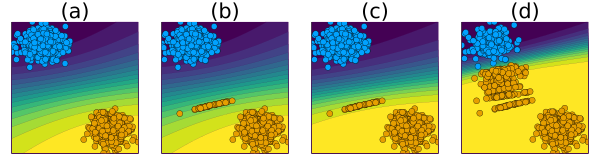
\includegraphics[width=0.45\textwidth,height=\textheight]{www/poc.png}

}

\caption{\label{fig-dynamics}Dynamics in Algorithmic Recourse.}

\end{figure}

\hypertarget{sec-related}{%
\section{Related and Future Work}\label{sec-related}}

\hypertarget{benchmarking-ce-in-julia}{%
\subsection{Benchmarking CE in Julia}\label{benchmarking-ce-in-julia}}

Until recently there existed only one open-source library that provides
a unifying approach to generate and benchmark counterfactual
explanations for models built and trained in Python (Pawelczyk et al.
2021). To address this limitation I have developed
\href{https://www.paltmeyer.com/CounterfactualExplanations.jl/stable/}{CounterfactualExplanations.jl}:
a Julia package that can be used to generate counterfactual explanations
for models developed and trained not only in Julia, but also in other
popular programming languages like Python and R. The package and
companion paper are currently pending acceptance for a main talk at
\href{https://juliacon.org/2022/}{JuliaCon}.

\hypertarget{probabilistic-methods-for-realistic-ce}{%
\subsection{Probabilistic Methods for Realistic
CE}\label{probabilistic-methods-for-realistic-ce}}

To ensure that the generated explanations are realistic it is important
to understand which input-output pairs are likely and which are not.
With respect to the work-in-progress presented here, I expect that this
may help in mitigating endogenous domain and model shifts. To quantify
the joint likelihood of input-output pairs, previous work has either
relied on generative models or restricted the analysis to probabilistic
models that incorporate uncertainty in their predictions. While the
former approach is more versatile, since it is applicable to both
deterministic and probabilistic models, the latter is computationally
much more efficient. The approach proposed by Schut et al. (2021) and
used to generate the examples in Figure~\ref{fig-dynamics} falls into
the latter category. In future work, I want to explore how recent
advances in post-hoc uncertainty quantification, most notably Laplace
Redux (Daxberger et al. 2021), can be leveraged to generate realistic
and unambiguous counterfactual explanations for any model.\footnote{For
  some initial work on this see my Julia implementation of Laplace
  Redux:
  \href{https://www.paltmeyer.com/BayesLaplace.jl/dev/}{BayesLaplace.jl}.}

\hypertarget{references}{%
\section*{References}\label{references}}
\addcontentsline{toc}{section}{References}

\hypertarget{refs}{}
\begin{CSLReferences}{1}{0}
\leavevmode\vadjust pre{\hypertarget{ref-daxberger2021laplace}{}}%
Daxberger, Erik, Agustinus Kristiadi, Alexander Immer, Runa Eschenhagen,
Matthias Bauer, and Philipp Hennig. 2021. {``Laplace Redux-Effortless
Bayesian Deep Learning.''} \emph{Advances in Neural Information
Processing Systems} 34.

\leavevmode\vadjust pre{\hypertarget{ref-joshi2019towards}{}}%
Joshi, Shalmali, Oluwasanmi Koyejo, Warut Vijitbenjaronk, Been Kim, and
Joydeep Ghosh. 2019. {``Towards Realistic Individual Recourse and
Actionable Explanations in Black-Box Decision Making Systems.''}
\emph{arXiv Preprint arXiv:1907.09615}.

\leavevmode\vadjust pre{\hypertarget{ref-karimi2021algorithmic}{}}%
Karimi, Amir-Hossein, Bernhard Schölkopf, and Isabel Valera. 2021.
{``Algorithmic Recourse: From Counterfactual Explanations to
Interventions.''} In \emph{Proceedings of the 2021 ACM Conference on
Fairness, Accountability, and Transparency}, 353--62.

\leavevmode\vadjust pre{\hypertarget{ref-mothilal2020explaining}{}}%
Mothilal, Ramaravind K, Amit Sharma, and Chenhao Tan. 2020.
{``Explaining Machine Learning Classifiers Through Diverse
Counterfactual Explanations.''} In \emph{Proceedings of the 2020
Conference on Fairness, Accountability, and Transparency}, 607--17.

\leavevmode\vadjust pre{\hypertarget{ref-pawelczyk2021carla}{}}%
Pawelczyk, Martin, Sascha Bielawski, Johannes van den Heuvel, Tobias
Richter, and Gjergji Kasneci. 2021. {``Carla: A Python Library to
Benchmark Algorithmic Recourse and Counterfactual Explanation
Algorithms.''} \emph{arXiv Preprint arXiv:2108.00783}.

\leavevmode\vadjust pre{\hypertarget{ref-schut2021generating}{}}%
Schut, Lisa, Oscar Key, Rory Mc Grath, Luca Costabello, Bogdan
Sacaleanu, Yarin Gal, et al. 2021. {``Generating Interpretable
Counterfactual Explanations by Implicit Minimisation of Epistemic and
Aleatoric Uncertainties.''} In \emph{International Conference on
Artificial Intelligence and Statistics}, 1756--64. PMLR.

\leavevmode\vadjust pre{\hypertarget{ref-upadhyay2021towards}{}}%
Upadhyay, Sohini, Shalmali Joshi, and Himabindu Lakkaraju. 2021.
{``Towards Robust and Reliable Algorithmic Recourse.''} \emph{arXiv
Preprint arXiv:2102.13620}.

\leavevmode\vadjust pre{\hypertarget{ref-ustun2019actionable}{}}%
Ustun, Berk, Alexander Spangher, and Yang Liu. 2019. {``Actionable
Recourse in Linear Classification.''} In \emph{Proceedings of the
Conference on Fairness, Accountability, and Transparency}, 10--19.

\leavevmode\vadjust pre{\hypertarget{ref-verma2020counterfactual}{}}%
Verma, Sahil, John Dickerson, and Keegan Hines. 2020. {``Counterfactual
Explanations for Machine Learning: A Review.''} \emph{arXiv Preprint
arXiv:2010.10596}.

\leavevmode\vadjust pre{\hypertarget{ref-wachter2017counterfactual}{}}%
Wachter, Sandra, Brent Mittelstadt, and Chris Russell. 2017.
{``Counterfactual Explanations Without Opening the Black Box: Automated
Decisions and the GDPR.''} \emph{Harv. JL \& Tech.} 31: 841.

\end{CSLReferences}

\end{document}
